\section{The File-system}\label{filesystem}

A working operating system cannot only function from ram. It needs a storage medium and with that there comes the need for a file-system. 

As my personal project, I did my best to use the functionality of the already implemented sdhc reader/writer and implemented parts of the fat32 file-system so that access to the inserted SDHC card is made possible. 

\subsection{Core Functionality \& Overview}
The terminology user is in the following chapter used equally to a process. 

The main purpose of the file-system and driver blackbox (for now at least) is to provide processes the access to a storage medium, the sdcard. With the access there comes the need for \emph{read}, \emph{write}, \emph{create} and \emph{delete} files and directories as well as retrieving the attributes they come with. 

The user can use this functionality by either including \C{<aos/fs\_service.h>} and use the commands 

\begin{mdframed}[style=myframe]
\begin{minted}[xleftmargin=\parindent,linenos,breaklines]{C}
void read_file(char *path, size_t size, char *ret);

void write_file(char *path, char *data);

void delete_file(char *path);

void read_dir(char *path, char **ret);

void create_dir(char *path);

void delete_dir(char *path);
\label{code:fsserv}
\end{minted}
\end{mdframed}

or just by using the following commands in josh (the shell). 

\begin{mdframed}[style=shell]
\josh{cat "\emph{path}"}

\josh{wtf "\emph{path}" "\emph{text}"}

\josh{rm "\emph{path}"}

\josh{mkdir "\emph{path}"}

\josh{ls "\emph{path}"}

\josh{rmdir "\emph{path}"}
\end{mdframed}

Please note that every path has to start with \C{"/sdcard"} as this is the requested root folder.

Now, this is a good place to talk about what my file-system is capable of. Sadly, it cannot do all the things I wished it could. I had to make some assumptions which I am going to talk about later on. The following list contains the functionalities I implemented successfully:

\begin{itemize}
\item Mounting the SDHC card at $/sdhc$
\item FAT32 entries are only of type \emph{short entry}
\item Creating files on the SDHC card
\item Reading files on the SDHC card
\item Writing at the end of files on the SDHC card
\item Truncate files on the SDHC card to a defined size
\item Creating folders on the SDHC card
\item Deleting folders on the SDHC card
\item Retrieving information on the folder/file on the SDHC card
\item No access conflicts with multiple processes on different cores
\end{itemize}

\subsection{Implementation}
The already implemented ram-file-system was a guideline for me and helped me understand how the connection between the c library call and the function call accessing the storage medium works. I am positive that I did not understand it completely. It was though a good example how important documentation is. 
At some later point in time it seemed a good idea to not only use the ram-file-system as a guideline but to follow the structure as rigid as possible. The reason for that was that I lost a lot of time in trying to understand the functionality/complexity of those calls and coming up with my own without any documentations on the inputs or output and I preferred a working system instead of some idea of a system.

To understand the fat32 format the fact-sheet provided was enough. Fascinating to see was that some things essential to me were missing when formatting the SDHC card on Linux. 

Here a small illustration how the pipeline works and therefore which parts the user needs to know about:

\begin{figure}[h]
    \centering
    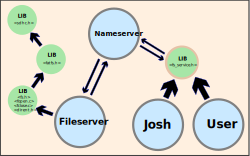
\includegraphics[width=0.9\textwidth]{./filesystem/data/fileaccess.png}
    \caption{Illustration of the file-system pipeline}
    \label{fig:ns_rtt}
\end{figure}

\subsubsection{FATFS library}
I implemented the main functionality/functions as a libraries of the file-system. They provide the connection between user and storage device. The communication (data transfer) between the SDHC driver and a server is done over the first slot in the ARG-CNODE. 

Important to note is the following terminology. The sdcard formatted as FAT32 consists in my case of clusters, which consists of sectors, which consists of bytes.

\subsubsection{Initializing/mounting}
The initialization consists of mounting the SDHC card to the folder "/sdcard" and connecting the fatfs functions to the c library function (fopen, fwrite, opendir, etc.). Mounting includes the creation of the \C{struct fatfs\_mount} which is crucial across all file accesses. 
The struct contains global information like the connection point to the sdcard (\C{struct sdhc\_s}), the directory entry for the root folder and the state of the FAT32 file-system (\C{struct fat32\_fs}). 

The state of the FAT32 file-system contains all info's about the FAT32 file-system inserted into the SDHC slot. Important to mention is the buffer page. It is an allocated frame mapped in the virtual address space, where the exchange between user and memory happens, the sdhc driver the connects the memory to the sdcard. The allocated frame is in my case not cached and therefore cache invalidation should theoretically not be necessary. 

With all these info's, manipulating bytes from/on the sdcard is possible.

\subsubsection{FAT Table-walk}
The FAT table-walk needs three operation types: 
\begin{itemize}
\item Retrieve the index of a free cluster
\item Get the next connecting cluster
\item Manipulate an entry
\end{itemize}

Thus only three functions are needed. In regard to retrieving a free cluster, all bytes in that cluster are zero'ed. It makes debugging as well as creating files in a cluster belonging to a folder less error-prone if your code is not perfect. As mine is not perfect, I encountered some conflicts with Linux formatting the sdcard, especially the root-folder. But more in the "Compromises / Encountered obstacles" section \ref{subsec:comp}.

\subsubsection{Directory-entries (dirent)}
A file or folder is always 32 Bytes on the FAT32 file-system and is called a directory-entry or dirent. Of course only under the assumption that there are only short FAT32 entries. On opening such an entry, a handle (\C{struct fatfs_handle}) is created containing the status and dirent info (\C{struct fatfs_dirent}) of the entry.

\begin{mdframed}[style=myframe]
\begin{minted}[xleftmargin=\parindent,linenos,breaklines]{C}
struct fatfs_handle
{
    struct fs_handle common;        ///< fatfs_mount pointer
    char *path;                     ///< string containing the path
    bool isdir;                     ///< offset in bytes
    struct fatfs_dirent *dirent;    ///< flag indication this is a dir

    off_t file_pos;                 ///< file content offset in bytes
    off_t dir_pos;                  ///< folder position offset in bytes
};

struct fatfs_dirent
{
    char *name;                     ///< name of the file or directory
    size_t size;                    ///< the size of the direntry in bytes or files
    struct fatfs_dirent *parent;    ///< parent directory

    uint32_t cluster;               ///< cluster number
    uint32_t sector;                ///< sector number
    uint32_t sector_offset;         ///< offset of sector to entry in bytes
    uint32_t content_cluster;       ///< cluster containing data or folder entries

    bool is_dir;                    ///< flag indication this is a dir
};
\end{minted}
\end{mdframed}

The name of an entry has an explicit length and way to be written into the FAT32 structure, therefore a translation between those two styles had to be done before comparing those two (useful when trying to find an entry).

\paragraph{File manipulation}
Regarding the fields contained in the handle struct and the ease of access to the entry on the sdcard, the functions \emph{open}, \emph{read}, \emph{write}, \emph{create}, \emph{truncate}, \emph{tell}, \emph{seek}, \emph{close}, \emph{stat} and \emph{remove} for files the implementation was not that simple as the operation the functions should perform was not clear. They were not intended to be called directly by the user but to be used by the standard c library functions. Those seemed to have an own agenda for what they use those functions and in the end it is still a mystery to me what some of those want from me.

In the case of writing, I made the assumption to only be able to write at the end of a file and therefore enlarging it. I did that regarding the time I had to understand the "blackbox" between the c library call and my function calls and the remaining time to come up with a working implementation.

Concerning the creation of a file: An empty file has no cluster containing the content. It is created as soon as the first write is attempted. 

Now comes the part where I thought I made a breakthrough understanding the c library calls. On reading, the function actually does not have to read the full required length. A small fraction suffices. The function calling my implemented read function is apparently a loop which calls my read function as long, as something readable is returned and concatenates the results. Therefore I was able to break down the implementation of the read function greatly into only reading chunks of a the size of a sector or until the sector-end.  

\paragraph{Folder manipulation}
Again, regarding the fields contained in the handle struct and the ease of access to the entry on the sdcard, the functions \emph{open}, \emph{create}, \emph{read\_next}, \emph{close} and \emph{remove} were equally problematic as those for files. 

On creating folders two "link-folders", namely "." and "..", are created. Those folders are only links and therefore don't have to be removed explicitly before removing a folder. The folder must though only contain those two link folders upon removal. 

\subsection{File-system-server or "Solving concurrent access"}
Now that the library was implemented, a server function which calls those functions seemed reasonably intelligent. This because then I had the problem of interfering concurrent accesses solved and it was not that complicated to implement. This compromise with on the other hand a loss in speed made the decision. 

The file-system-server is connected to the name-server and awaits incoming file-access-requests. Including a handler function, which handle incoming file-access-requests, the server also initializes and mounts the file-system. Important to note is that the init-process has to wait until the server registered the handler on the name-server. Otherwise file-access-requests grant an error. 
I went for the registration of a handler function on the name-server over an RPC-call because the connection between caller and callee is direct and the interface matches the requirements of the file-system-server.

\subsection{File-system service}
The file-system service implemented as a library in \C{<aos/fs\_service.h>} connects the user (over the name-server) with the file-system-server. These \ref{code:fsserv} functions allow him to access the file-system on the sdcard. 

Interesting to point out is that the message sent over the name-server has always the same structure. The type field sent along the message is the identifier what the call actually should execute on the other side and also defines the return value.  

\subsection{Compromises / Encountered obstacles}
\label{subsec:comp}

\subsubsection{SDHC reads and the Cache}
As mentioned before, the allocated frame, which connects the user to the ram is not cached. Unfortunately there were some delays between reading/writing and accessing the the read bytes from the sdcard on the memory. I did not find out why it had delays. Invalidating the cache before a read with a memory barrier or flushing the cash before a write with a memory barrier had no effect. 
I encountered this problem as I removed the \C{debug\_printf} statements and imitated those delays with an volatile for-loop. This fix is ugly but it does the trick (for now).

\C{for (volatile int t = 0; t < 1000000; t++);}

Analysing this bug was a dead end. The label \C{NOCACHE} was successfully loaded into the pagetable and debugging the sdhc driver was not successful as the debug messages showed no sign of failure.

\subsubsection{Formatting on Linux}
Interesting to see was that formatting on Linux did not set the cluster containing the entries in the root folder to zero or delete the files in it. This was quite the hustle, as I thought I did something wrong but it seemed the attribute was set to zero. It is still quite a mystery to me, what Linux understands under formatting. The specs sheet of FAT32 clearly commands you to set all entries in a newly assigned cluster for a folder to zero.

\subsection{Measurements/Performance}
I did some measurements on the function call writing and reading to the sdcard (\C{<sdhc.h>}). For stability reasons I performed the following measurements 100 times.
\begin{itemize}
\item Sequential sdhc\_read: 475ms
\item Sequential sdhc\_write: 475 ms
\item Alternating sequential read/write's: 955 ms
\end{itemize}

This indicates, that on switching from read to write or vice versa, 5 ms are lost somewhere. 

Now comes the interesting part. I measured the fastest time for each file-system call (\C{fs\_service.h}). 
After 10 iterations it was clear, that the values are always the same.
Important to note is, that writes and reads with large content increase in time, every new sector. This makes sense as every new sector has to be loaded and written to the sdcard.

\begin{itemize}
\item Sequential write\_file (incl. creation): 924 ms
\item Sequential read\_file:  90 ms
\item Sequential remove\_file: 406 ms
\item Sequential create\_dir: 863 ms
\item Sequential read\_dir: 172 ms
\item Sequential remove\_dir: 341 ms
\end{itemize}

The quick-fix for the sdhc driver increases the time for every read/write from/to the sdcard by 20 ms. 

Now, the attentive reader may have noticed, that the "Sequential sdhc\_read" take way more time than the direct "Sequential read\_file". But it should not! The "Sequential sdhc\_read" is called in the "Sequential read\_file", so the later should take more or equal the amount to time of the first. The only way I can think of explaining this phenomenon is that the first measurement is called right after initializing the file-system and the second one is called from user space. Therefore some optimizations/caches probably happen between those two calls. 

\subsection{Improvements}
This is clearly not best solution for implementing a file-system. I would even go as far as it is not even a good one. Improvement can be done from the beginning. I will not go into functionalities which I did not implement. Concerning speed, the sdhc bug would give us some speedup. But it is not significant. More interesting I think is that most of the time is lost due to the read and writes to and from the FAT table and FOLDER ENTRIES to the same sectors. Thus a cache or a bigger buffer (currently only one sector) would in most cases result in a speedup. The principles of temporal locality and spacial locality can be applies to storage media (at least at some scale).

All in all this could bring some speedup but the worst case remains the same. 

Furthermore understanding the c lib function calls will help to further break down my implemented functions to a simpler constructs with possible speed gain. The other way is also possible, instead of breaking down the functions, implement an algorithm which solves the request directly. I am thinking of the \C{fatfs_read} function, where I only return chunks of the requested file. If I returned the full requested read size, then the usage of the buffer-page will be better.

Concerning work allocation, right now there is only one process managing the whole file-system. I could imagine some speedup if there were multiple processes for managing the FAT, the DATA section or even each individual function calls. As interesting this sounds, the problems it comes with are another hurdle. With this idea, concurrency and race-conditions become a real problem and the concept has to stand before one can even attempt to program such a structure. 